
I denne delen skal jeg introdusere de ulike typene relevant erfaring man kan få, hvordan man skaffer dem og hvor man finner disse stillingene. Jeg har valgt å dele det inn i fem kategorier:

\begin{enumerate}
    \item Summer internship
    \item Winter internship
    \item Ferievikarer
    \item Deltidsjobb ved studiene
    \item Kurs og caser
\end{enumerate}

Dette er noe som allerede 1.-klassinger kan kikke på, fordi flere kurs og opplegg krever at man er tidlig i studieløpet. Ved å vite om dette på forhånd kan man unngå å gå på en smell senere.


\section{Summer intership}

Jeg kommer til å bruke navnene summer internship, internship og sommerjobb om hverandre. Kjært barn har mange navn, men summer internship høres mer fancy ut.

Det første du trenger å vite, er at summer internships lyses ut på typiske jobbsøkeportaler som Finn og LinkedIn. Ofte er selskapene ute etter studenter i 3. og 4. klasse på grunn av progresjonen i studiet. Dette handler både om kunnskapene man besitter og om når de kan ansette deg! Jeg deler summer internships inn i to kategorier: bedrifter som bruker det som ekstra arbeidskraft i sommerperioden og bedrifter som bruker det som en intervjuprosess.

Den første kategorien fungerer i praksis som vikariater, hvor studentene løser små oppgaver de faste ansatte ikke har rukket å gjøre. Sommerferien er ofte en tid de fleste tar ferie, og siden mange bedrifter har oppgaver de gjerne skulle ha utført selv, overlater de derfor dette til studentene.

Den andre kategorien gir studentene egne prosjekter, som for eksempel en kundecase i et konsulenthus eller utforsking av nye ideer. I disse stillingene produserer studentene i varierende grad noe nyttig for bedriften og det handler mer om å finne de aktuelle studentene for en fast stilling. Derfor er en internship-stilling perfekt for en slik bedrift her, ettersom det er en 2 måneder lang intervjuprosess, men med ingen forpliktelse om å ansette vedkommende etterpå. Husk at dårlige ansatte koster mer enn å ansette sommerstudenter.

Når det gjelder intervjuprosesser, finnes det mange ulike metoder som bedrifter benytter. De fleste krever et motivasjonsbrev, CV og ofte karakterutskrifter. Store selskaper som Equinor har lange og tidvis krevende prosesser, hvor man må gjennom CV-sjekk, evnetester, automatiske videointervjuer og eventuelt et avsluttende intervju. Mange lurer på hvilke spørsmål som blir stilt under intervjuene, men dette er vanskelig å forutsi. Automatiske videointervjuer har ofte standardiserte spørsmål, så hvis en venn har tatt det før, er spørsmålene sannsynligvis de samme. Dette er nyttig å vite, siden du har begrenset med tid til å svare når spørsmålene dukker opp. 

Jeg vil også påpeke at konsulentbransjen ofte har de mest utfordrende intervjuene, hvor de kan stille tilsynelatende absurde spørsmål. For eksempel kan du bli spurt: <<Hvor mange golfballer får plass i en Boeing 747?>> eller <<Hva er markedsandelen til iPhone i India?>>. Det kan virke skremmende, men såkalte <<Guesstimates>> blir mye enklere å håndtere med litt øvelse. Det finnes mange guider som kan hjelpe deg med å løse slike oppgaver, noe jeg vil gå nærmere inn på senere.

\begin{remark}
    \textbf{OBS OM FRISTER} Sommerjobber har varierende frister, så det er viktig å starte søknadsprosessen tidlig, gjerne i august. Konsulenthus har ofte tidlige frister, mens større kjemirelaterte stillinger kommer i september/oktober og våren. Opprett varsler på Finn og LinkedIn med søkeordene: \textit{summer intern}, \textit{summer internship}, \textit{sommerjobb ingeniør} og \textit{sommerjobb teknisk}. Mange stillinger har fortløpende opptak, så søk tidlig. Det anbefales å ikke ta for mye hensyn til fristene da mange stillinger har fortløpende opptak uten å nødvendigvis nevne det.
\end{remark}

Historisk sett har det vært vanlig å søke både fulltidsjobber og sommerjobber i løpet av våren. Det kan virke merkelig å ansette en student allerede i september for en jobb som ikke starter før juni, men bedriftene har blitt stadig mer ivrige etter å sikre seg de beste kandidatene så tidlig som mulig. Dette handler ikke nødvendigvis om å få tak i de mest akademisk dyktige, men heller om å finne de mest motiverte som søker tidlig. Nylig har noen selskaper presset søknadsfristene så langt frem at de gikk ut allerede i august, noe som mange synes er urimelig. Som respons truet linjeforeningen Abakus med å kutte samarbeidet med bedrifter som opererte på denne måten, noe som førte til at fristene ble flyttet tilbake til september/oktober.

Det som derimot ikke snakkes så høyt om, er at mange stillinger nå har fortløpende søknadsfrister. Det vil si at hvis du søker på den oppgitte fristen i annonsen, kan det allerede være for sent. Selskapet kan ha sendt ut tilbud til flere kandidater før søknaden din i det hele tatt blir vurdert. Jeg har selv opplevd dette med en sommerjobb jeg var svært interessert i, men ventet for lenge med å søke på. Derfor er det viktig å være oppmerksom på fristene og søke i god tid.

\begin{remark}
    \textbf{HVORDAN LAGE CV} Det finnes mange fine CV-maler på Word og Overleaf, bruk dem. Tekna har også en CV-bygger med søknadsbrev som jeg har brukt. Skaff deg også LinkedIn, mange HR-folk liker å kikke på profilene til folk her. Her kan man også få lagt inn det man eventuelt ikke får plass til på CV-en. Legg ved LinkedIn-profilen din på CV-en. Skal du være enda mer fancy kan du lage din egen nettside, har du klart ITGK klarer man fint å lese seg opp på det, men er kanskje for de spesielt interesserte. 
\end{remark}

Det er verdt å bruke tid på CV-en sin, men legg merke til at det oftest bare tar tid den første gangen. Når CV-en har blitt laget så er vedlikeholdsprosessen mye lettere. Jeg ville heller fokusert på å bruke mer tid på å søke på stillingene, og et typisk tips er å lese annonsen nøye. Alt er der for en grunn, uavhengig om du forstår deg på det eller ikke. Det var flere ting jeg ikke skjønte med annonsen før jeg startet i internshipet, men først da ga det mening. Eller så burde jeg bare gjort mer research, hvem vet. Jeg ville også brukt LinkedIn til å finne hvem som hadde tilsvarende stilling i fjor og spurt om tips, ettersom de ofte vet hvilke spørsmål som stilles og hva HR fokuserer på. 

\begin{remark}
    \textbf{BILDE ELLER IKKE?} Det er et evig spørsmål om CV-en skal inneholde et bilde eller ikke. I England er dette en no no, men jeg ville ha oppfordret folk til å ta med bilde. Sett deg selv i skoene til en i HR, det er mye lettere å huske et fjes enn en CV. I den anledning ville jeg anbefalt å dra på CV-fotografering med Kjemidagen eller Tekna, begge er gratis! Eller så kan man spørre folk som er flinke til å ta bilder, de i Promokom kan ofte stille opp på kort varsel ;)
\end{remark}

Jeg vil også understreke hvor raskt folk kan eliminere seg selv fra en stilling ved å tro at de ikke oppfyller alle kvalifikasjonene. Det er viktig å huske at mange av de oppførte <<kvalifikasjonene>> ofte er veiledende, og hvis du klarer å selge deg selv godt nok, har det mindre betydning om du ikke oppfyller hver eneste en. Jeg fikk for eksempel et internship i et selskap som jobber med vannkraft, til tross for at jeg ikke hadde noen forkunnskaper om vannkraft (svaret er ingenting). Dette viser hvor mye motivasjon og personlighet betyr.

Selv om en stilling er merket som forbeholdt 4. klassinger, bør du likevel søke – kanskje får du den, og i verste fall har du bare brukt litt tid på søknaden. Hvis du er så heldig å få et internship tidlig og lurer på om det er verdt å søke i 4. klasse, er svaret mitt: absolutt! Som 4.-klassing blir du automatisk prioritert høyere enn 3.-klassinger, ikke nødvendigvis på grunn av mer erfaring, men fordi du er nærmere ferdig. For en arbeidsgiver fungerer et internship ofte som et forlenget intervju, og det er vanlig praksis i mange selskaper å tilby fast jobb eller deltidsjobb etter endt internship. Derfor bør du virkelig prioritere å søke internships i 4. klasse, for da har du kanskje sikret deg en fast jobb allerede før 5. klasse. Dette er en svært vanlig praksis blant konsulenthus, og litt mindre vanlig hos kjemibedrifter.




\section{Winter internship}

Ikke tro at sommerferien er den eneste perioden hvor du kan få internship! Selv om sommerferien er tiden hvor de fleste har fri, er det også vanlig med <<Winter internships>> rundt januar/februar. For mange bedrifter er dette faktisk mer gunstig, siden alle ansatte er på jobb, noe som gjør det lettere å følge opp studentene. Om sommeren kan ferieavvikling skape utfordringer, og derfor er noen bedrifter mer usikre på å tilby sommerjobber, fordi de må ha folk tilstede for å veilede studentene. Dette er vanlig praksis i konsulentbransjen, men mindre utbredt i industrien. Det betyr imidlertid ikke at mulighetene ikke finnes – ta kontakt med ansatte i bedriftene du er interessert i og spør om mulighetene!

Winter internships kan også være svært gunstige hvis du planlegger utveksling på våren, spesielt hvis semesteret er litt annerledes. For eksempel starter vårsemesteret i Italia i slutten av februar med eksamensperiode i juni/juli. Da kan det være vanskelig å få sommerjobb, men det gir en perfekt mulighet til å jobbe i januar/februar. Dette kan også åpne dører til flere muligheter senere. 


\section{Ferievikarer (perfekt for 1.klassinger!)}

Internships er ofte rettet mot studenter som har kommet et stykke ut i studiet, men det mange ofte glemmer er muligheten til å bli \textit{ferievikar}. Dette er stillinger som ikke nødvendigvis krever at man har kommet langt i studieløpet. Jeg tenker spesielt på stillinger som operatør hos bedrifter som Hydro, Elkem, vann- og avløpsetater, og lokale industriselskaper. Mange av disse stillingene er såpass enkle at selv videregående elever kan klare dem. For eksempel ansetter Hydro rundt 600 ferievikarer over hele Norge. Disse stillingene er godt betalt, på nivå med deres summer internships, og de blir godkjent som relevant erfaring.

Det som gjør MTKJ-studenter spesielt ettertraktede er vår solide forståelse for teknologi, grunnleggende prosesskunnskap, og kjemi. Dette gjør ferievikarstillinger hos Hydro til en perfekt mulighet for alle MTKJ-studenter.

Personlig angrer jeg veldig på at jeg ikke visste om denne muligheten tidligere. Som østlending hadde det vært utrolig spennende å for eksempel flytte til Vestlandet for en sommer, samtidig som jeg hadde hatt en interessant og relevant sommerjobb. 

\begin{figure}[H]
    \centering
    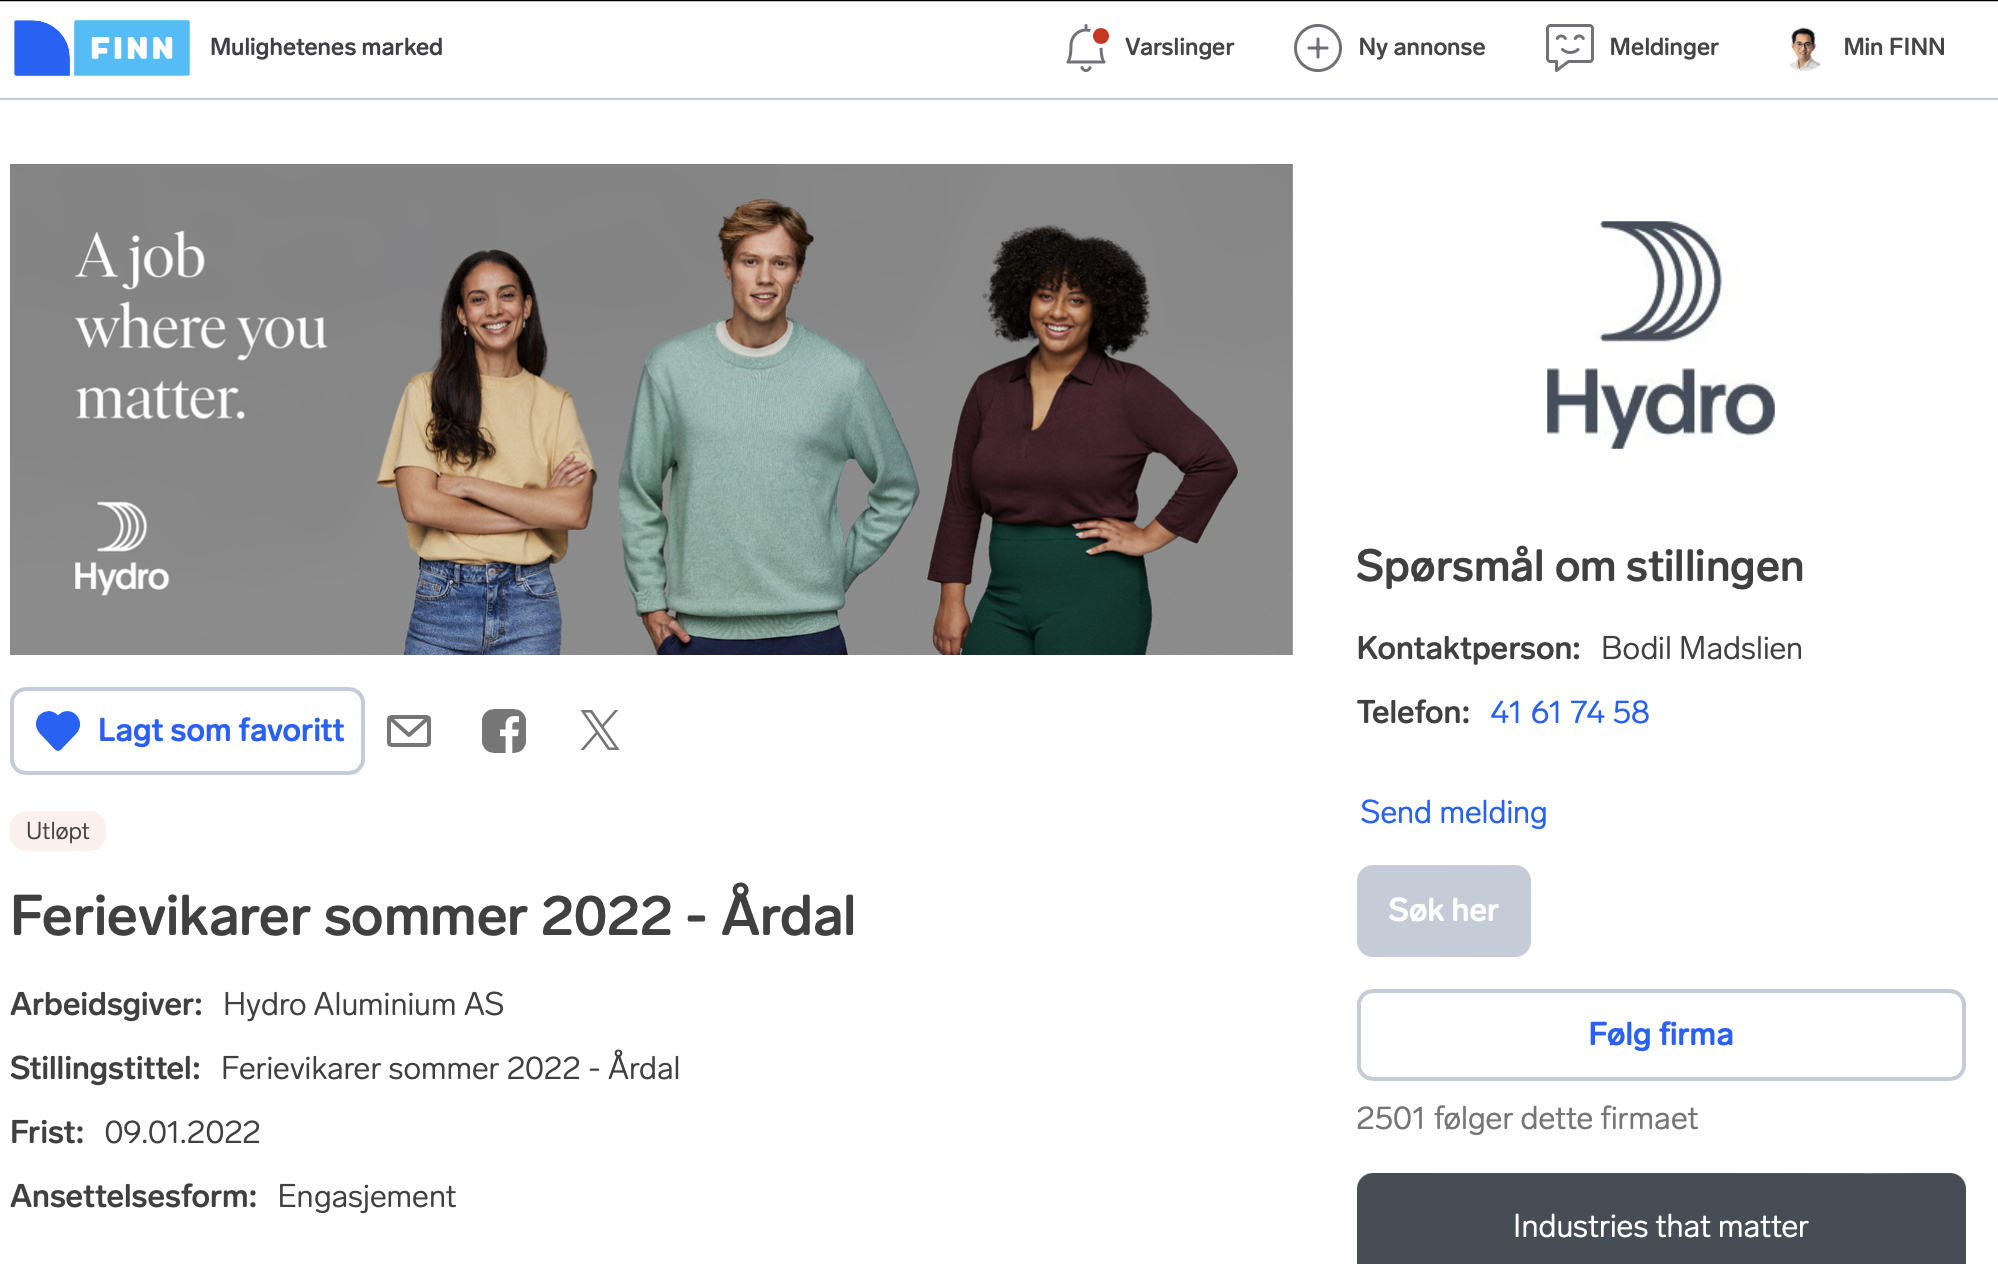
\includegraphics[width=1\linewidth]{images/hydro.png}
    \caption{Ferievikarstilling fra Finn.no}
    \label{fig:Hydro-annonse}
\end{figure}


\section{Deltidsjobb ved studiene}

De enkleste deltidsjobbene å få er ofte hos NTNU. Hvis du er interessert i å bli labassistent, kan du spørre foreleserne om de trenger hjelp i laboratoriet. For dem er det ofte billigere å bruke en student enn å sette en PhD-student på oppgaven. Dette kan føre til både en deltidsjobb under studiene eller en videreføring til en sommerjobb.

Den aller enkleste måten å få en deltidsjobb på, er å bli studassistent. Det er en myte at du må ha A i faget for å bli studass. Det handler mer om å være strategisk. Ja, hvis mange søker på stillinger i Generell kjemi, blir det ofte A-studentene som får jobbene, men husk at det finnes mange andre kjemifag. Flere sivilingeniør- og ingeniørstudier har kjemi eller basisfag som en del av pensum. Da kan det for eksempel holde med en C for å bli studass for byggstudenter. Du kan også bli studass i forkurs, som dekker grunnleggende videregående kjemi. Derfor anbefaler jeg at du ser gjennom alle studass-stillingene – det finnes alltid noen stillinger som ansetter bredere. Ikke alle fag har studass-opplegg på nivå med ITGK og matte.

Det er også viktig å få din første studass-stilling. Alle som blir studass må ta et kurs ved NTNU som heter LAOS-kurset. Når du har tatt dette kurset, blir det lettere å få din neste stilling, siden de ikke trenger å betale deg like mye som søkere uten LAOS-kurs. Du kan også få LAOS-kurs ved å være Teknostart-studass, så det er absolutt verdt å søke der også.



\section{Kurs og caser}

Dette er min favorittkategori fordi det rett og slett er gøy. Det kan virke litt overambisiøst å lete etter kurs eller casekonkurranser og deretter søke på dem, men la oss ta en titt på hva det egentlig handler om.

La oss begynne med kurs. Det finnes utallige kurs du kan søke på. NTNU har mange samarbeid med utenlandske universiteter, noe som gir deg muligheten til å få finansiert for eksempel en uke med studiepoenggivende kurs i Hellas. I tillegg finnes det kurs arrangert av bedrifter, som Bearingpoints konsulentskole. Hvis du er jente (som de fleste på MTKJ er), kan du også prøve deg på McKinseys program rettet mot unge kvinner.

\begin{figure}[H]
    \centering
    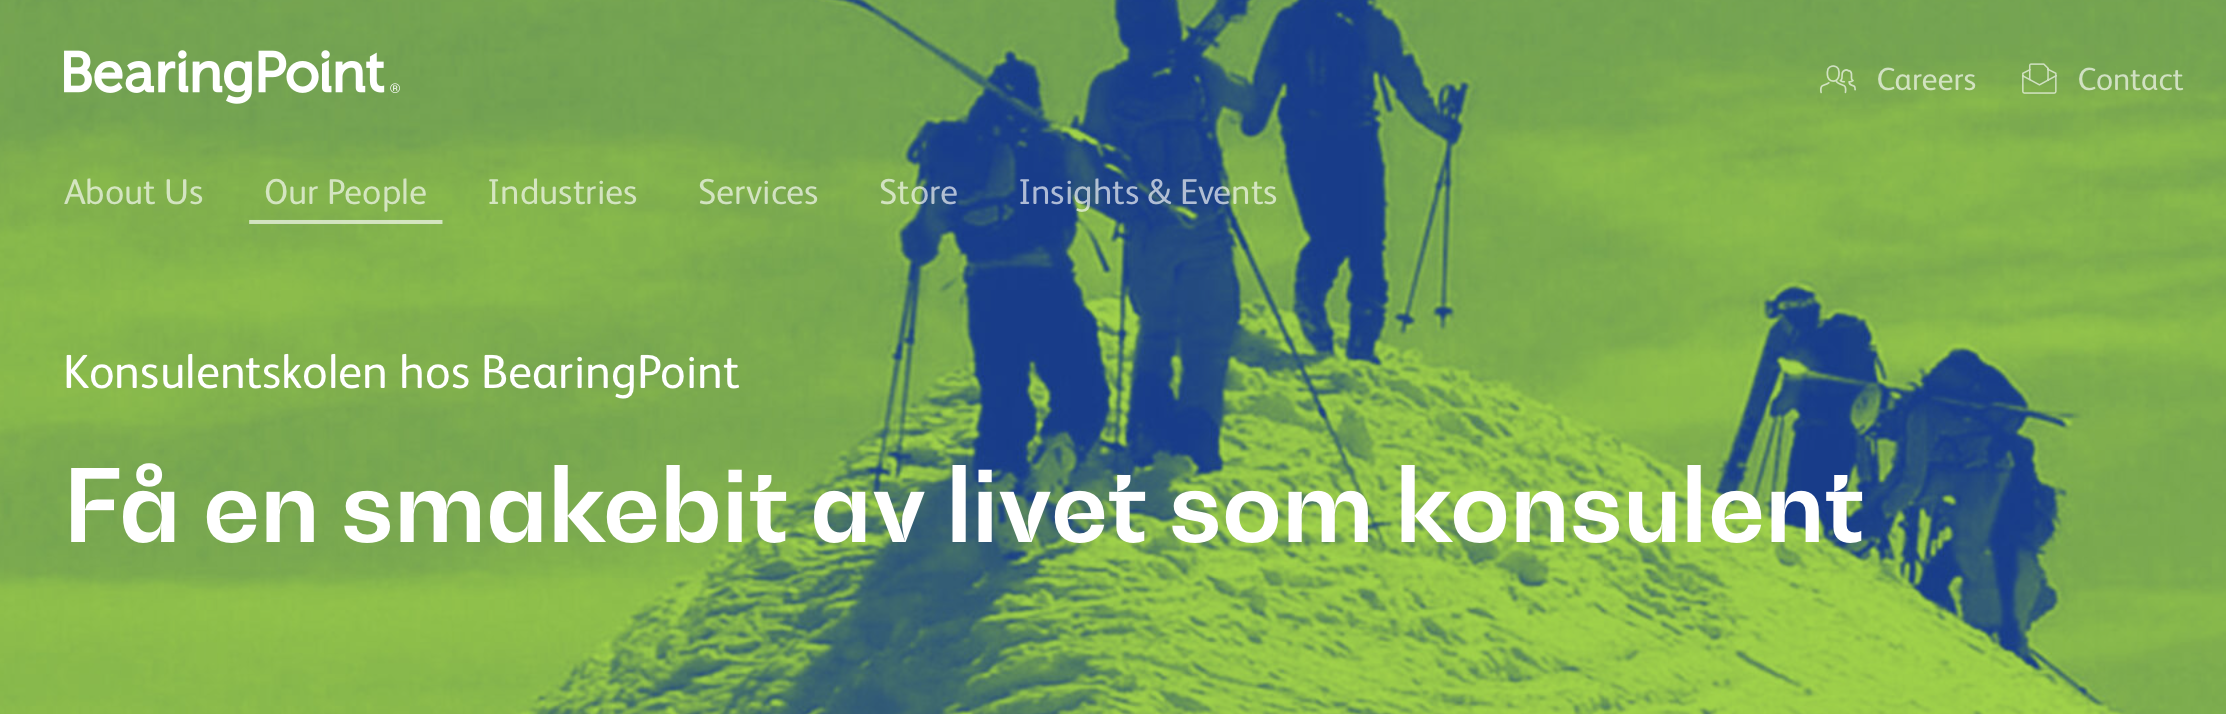
\includegraphics[width=1\linewidth]{images/bearingpojnt.png}
    \caption{Bearingpoint som konsulentskole, verdt å kikke på}
    \label{fig:Beairngpoint}
\end{figure}

\begin{figure}[H]
    \centering
    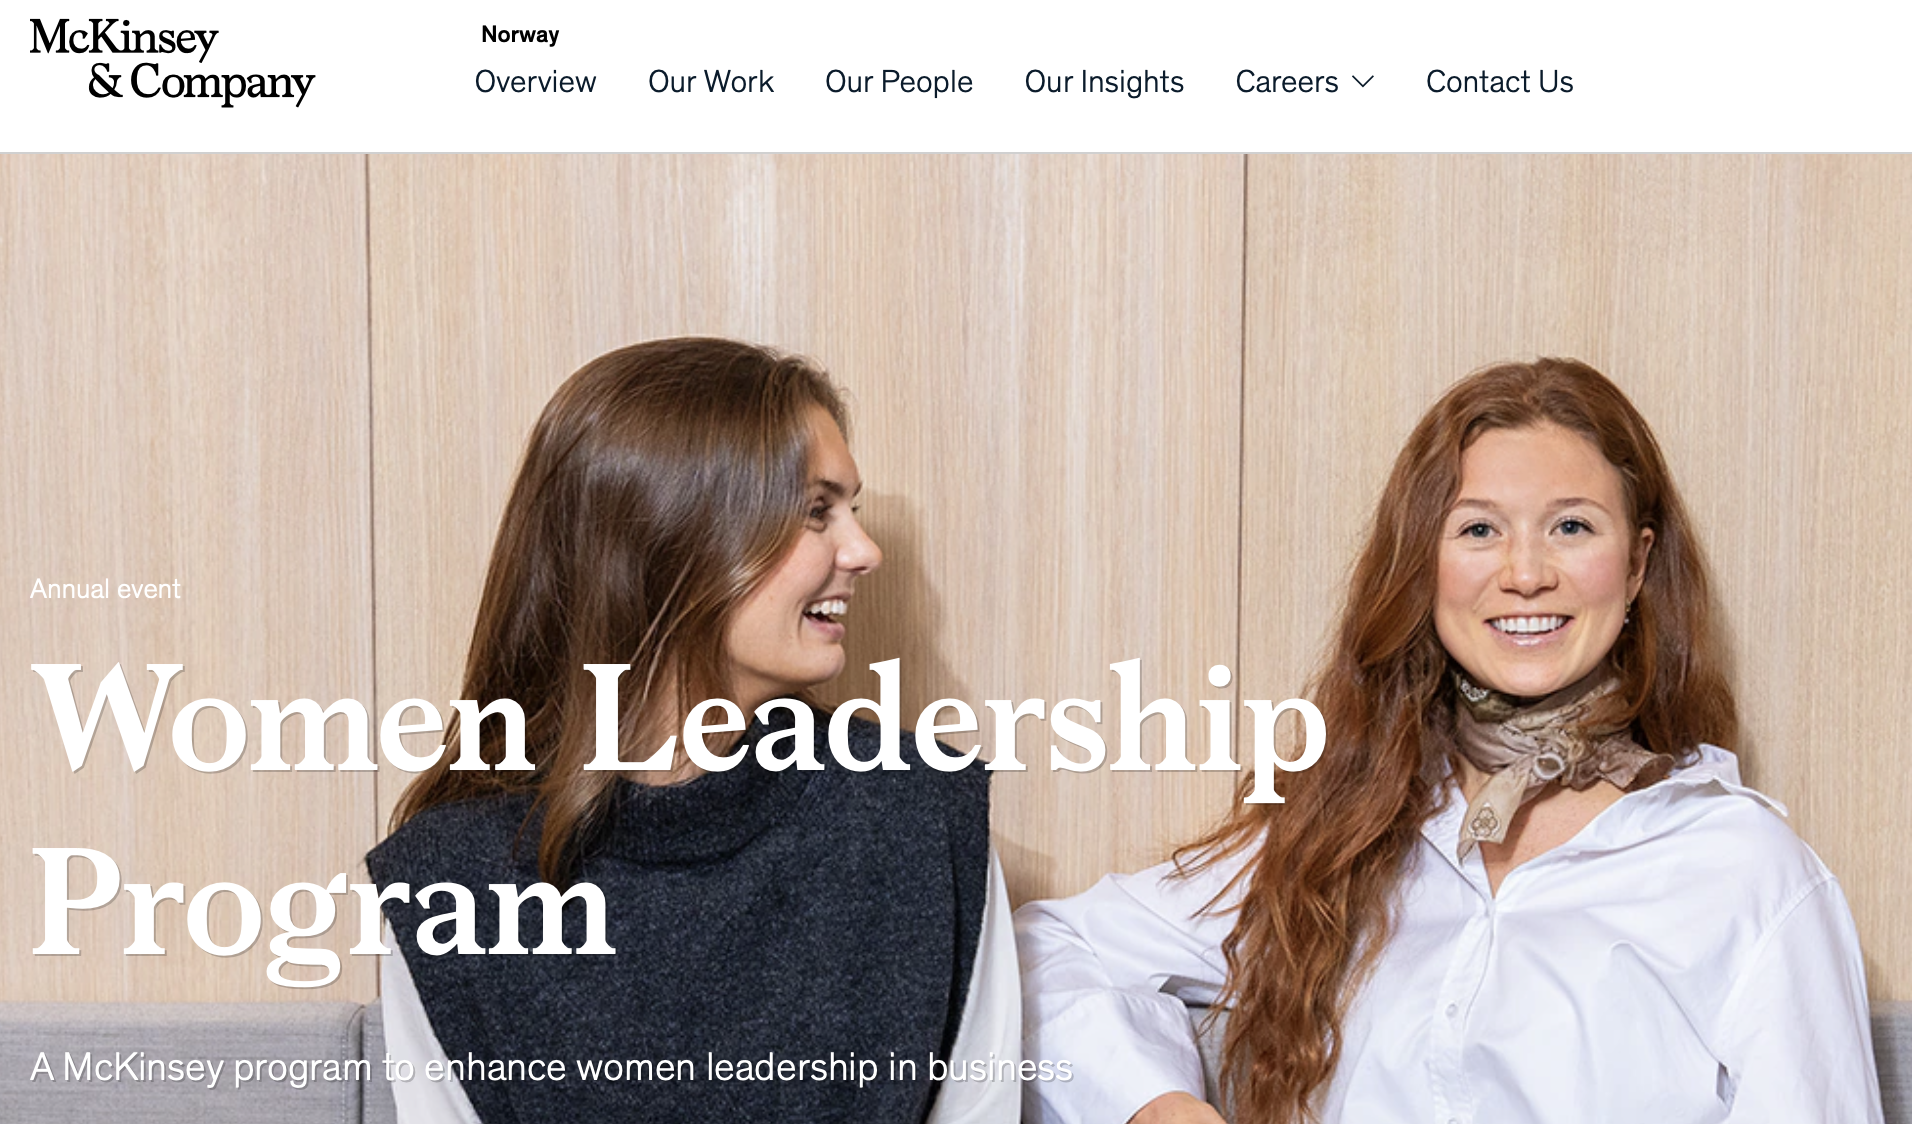
\includegraphics[width=0.8\linewidth]{images/mckinsey.png}
    \caption{Women Leadership Program}
    \label{fig:enter-label}
\end{figure}

Nå skal jeg snakke spesifikt om casekonkurranser. Disse kan ofte oppfattes som slitsomme, men det er egentlig ikke tilfellet! En typisk casekonkurranse går ut på at man får begrenset med tid til å løse et problem som ofte virker umulig. Det handler imidlertid mer om å tenke utenfor boksen og vise juryen hvordan din løsning er unik – du trenger ikke nødvendigvis å finne opp en ny kreftmedisin, liksom. 

Men la oss være ærlige, man deltar ikke på casekonkurranser bare for moro skyld, men også for fordelene de gir. Så hva er det egentlig man kan få ut av det? Jeg skal liste opp noen av disse konkurransene og hvilke goder de tilbyr i Tabell \ref{tab:Casekonkurranser}. Det finnes mange flere, men dette er de jeg har mest erfaring med.

\begin{table}[H]
    \centering
    \begin{tabular}{p{3cm}p{10cm}}
        \toprule
        Event & Innhold \\
        \midrule
        Aker Talent & Reise tur-retur Oslo inkludert hotellopphold, mat (+ drikke hehe), og sosialt opplegg som curling. Varer i 2 dager. Premien er litt uklart da det varierer fra år til år, men svært mange blant deltagerne får tilbud om sommerjobb eller fulltidsjobb fra et av Aker-selskapene (og det er heldigvis mange!). \\
        
        Skanska Grensesprenger & En av de lengre casene hvor man lager et lag selv og løser oppgave på egen tid. Premien er derimot ganske syk, fordi de sletter studielån opptil 165 000 kr for alle på vinnerlaget. \\
        
        Norconsult Hunger Games & Høres weird ut, men faktisk ganske artig med ulike aktiviteter osv. Det er hovedsakelig bygg, EMIL og maskinstudenter, men som MTKJ har man muligheten til å skille seg ut. Det foregår på kveldstid over to dager i Trondheim så ikke like intenst som andre. Det er selvfølgelig middag og drikke inkludert. Man blir heldigvis eliminert i puljer, så man ikke trenger å føle seg dårlig (jeg røk ut i første pulje). Vinneren får tilbud om fulltidsjobb hos Norconsult. Det du derimot ikke får vite, men som er svært viktig, er networkingen som skjer underveis. Det er 50 deltagere og like mange representanter fra Norconsult tilstede. De gjør ikke dette fordi penger er lættis, men fordi de er ute for å kikke etter folk. Dette gjør at noen kan ryke ut første runde, men likevel få sommerjobb den neste uken bare av å snakke med folk. \\
        
        Clara Idéathon & Du blir flydd til Bergen med hotell og alt sammen, ligner veldig på Aker Talent. Clara var derimot mindre skummelt siden det ikke var like mange tilskuere som på Aker Talent. \\
        
        Kongsberg Your Extreme & En konkurranse som arrangeres av Kongsberg ved NTNU og USN (Kongsberg, duh). Premien er på 100 000 kr , og det fine her er at alle deltagere blir invitert til en gallamiddag på Scandic Lerkendal. Så worst case er en 3-retters middag. \\
        
        AF-kollektivet & En årlig konkurranse hvor premien er å bo gratis i et år. Det huset vinnerlaget får er ganske gigantisk, så det er absolutt verdt tiden man investerer. \\
        \bottomrule
    \end{tabular}
    \caption{Oversikt over noen casekonkurranser}
    \label{tab:Casekonkurranser}
\end{table}

\begin{figure}[H]
    \centering
    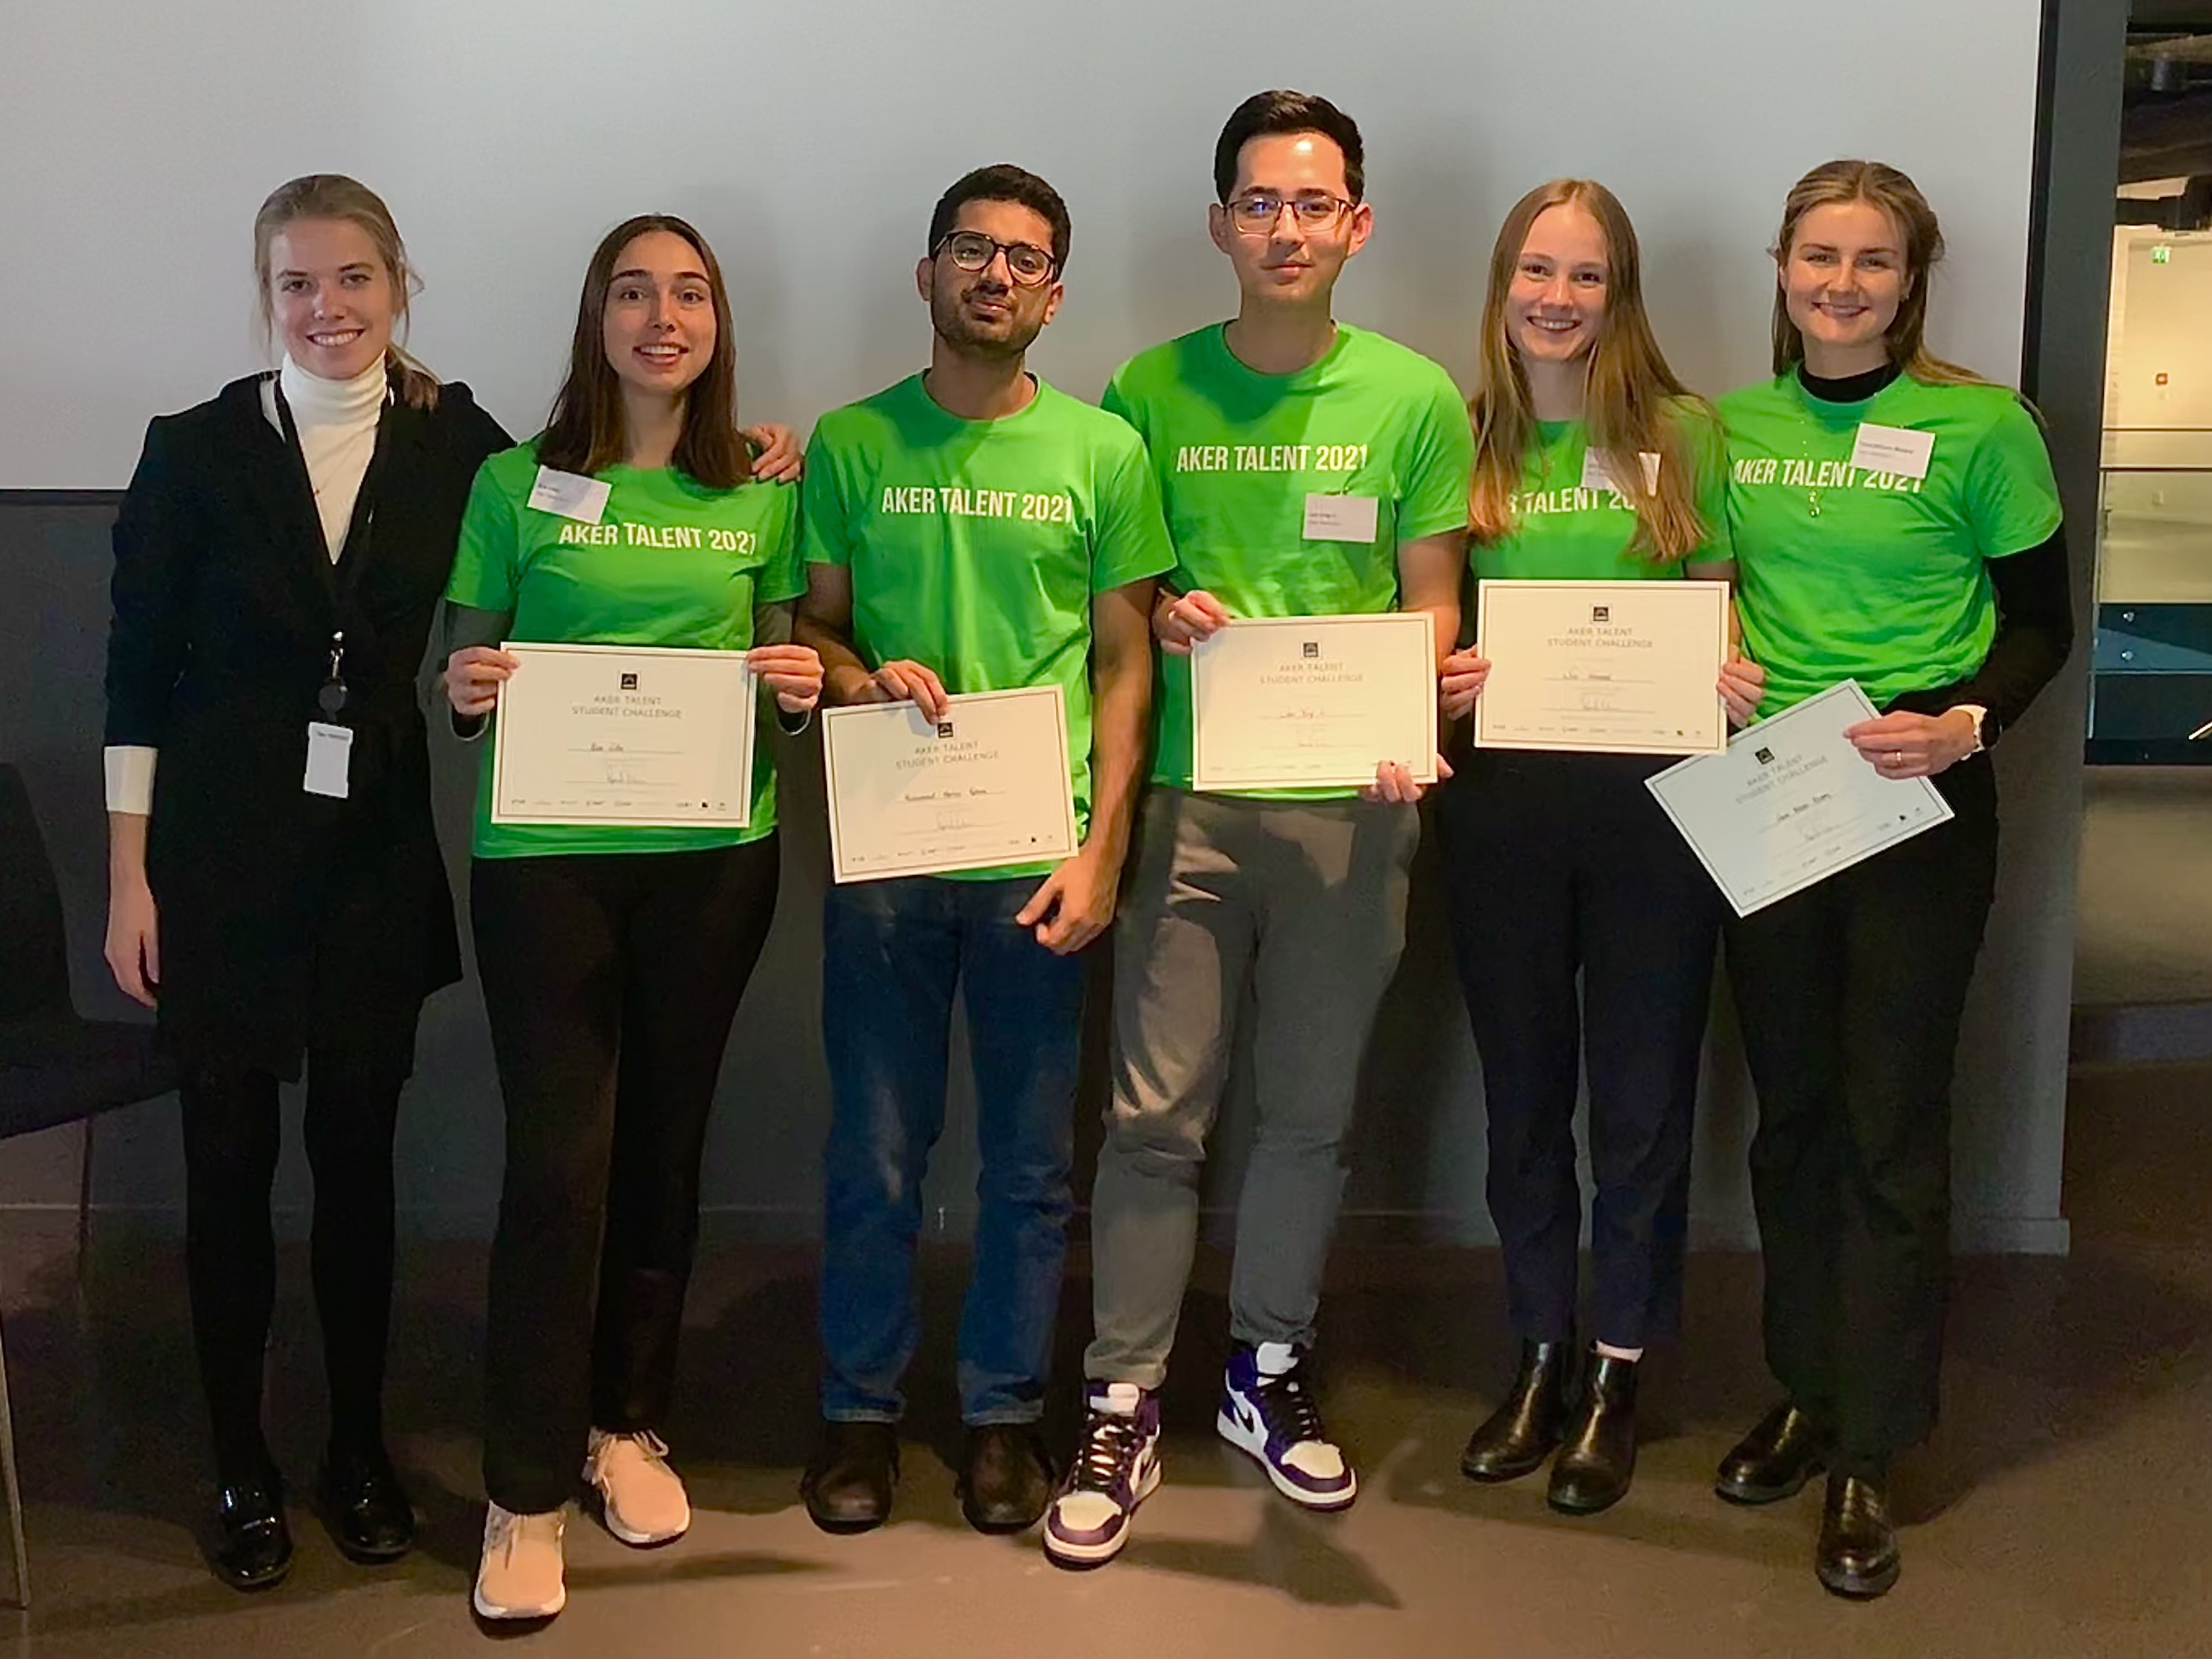
\includegraphics[width=0.6\linewidth]{images/Aker.jpg}
    \caption{Xing på Aker Talent, han høyeste med Jordans.}
    \label{fig:Aker}
\end{figure}

\begin{figure}[H]
    \centering
    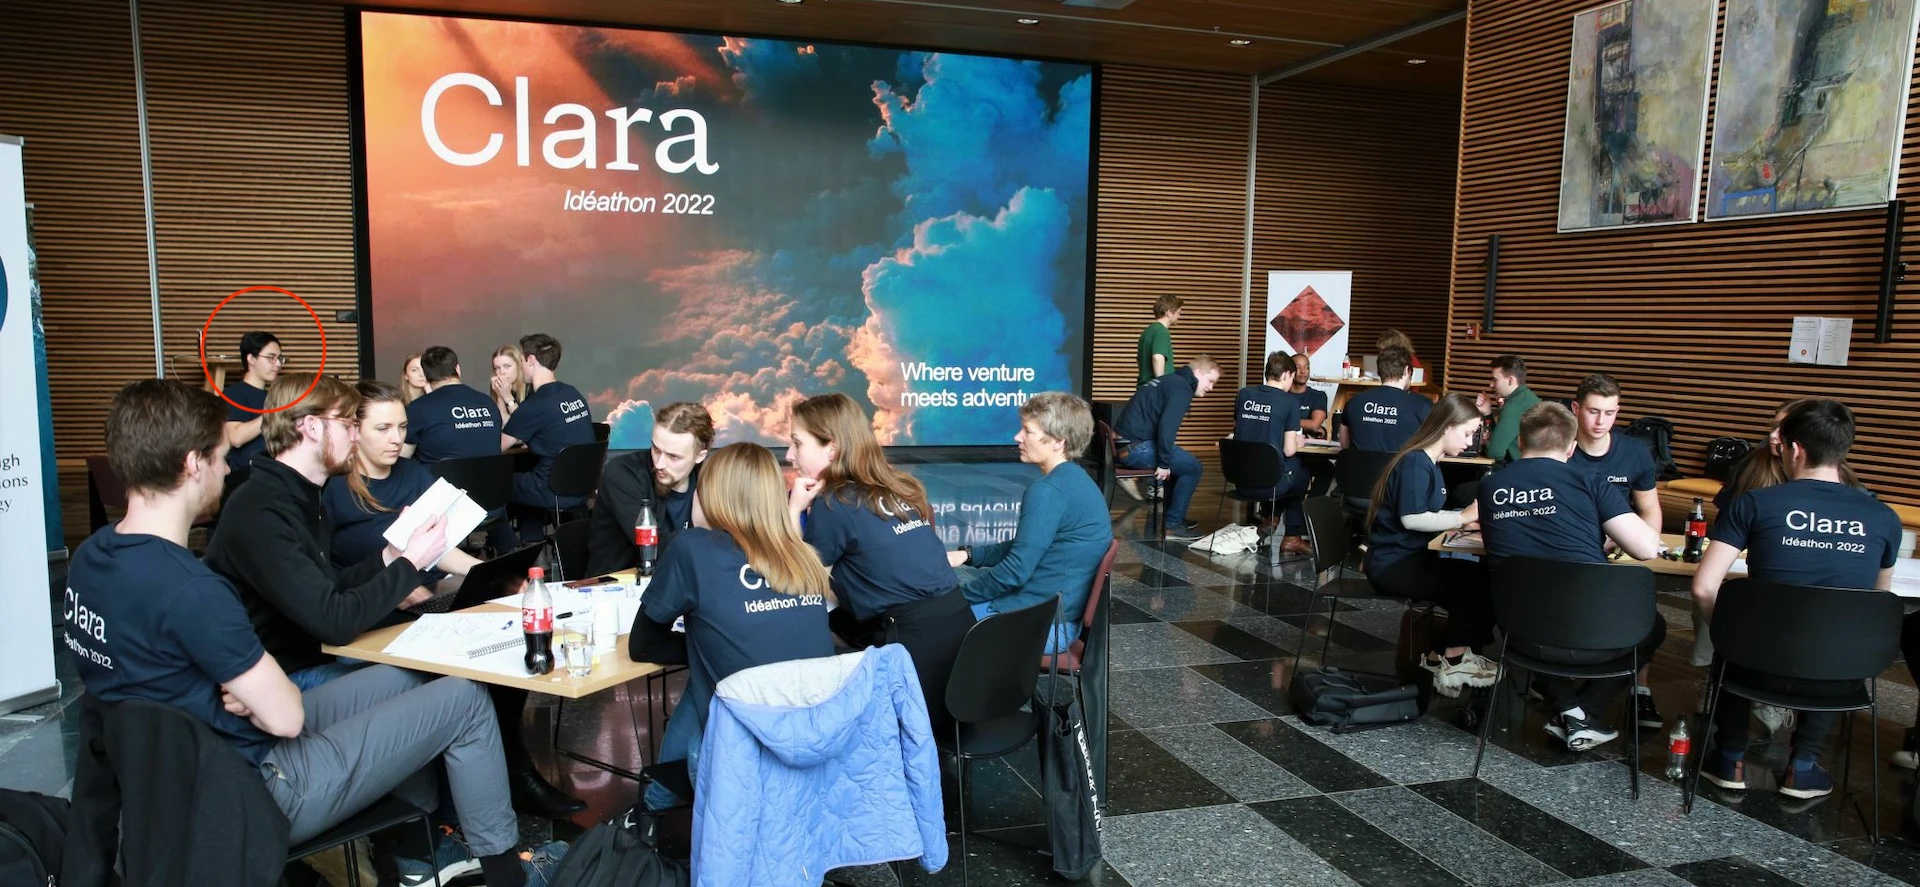
\includegraphics[width=0.8\linewidth]{images/Clara.jpg}
    \caption{Xing på Clara Idéathon, rød sirkel.}
    \label{fig:Clara}
\end{figure}

